\section {Stavba pulzního oxymetru}
\subsection {Volba platformy}
Jednou z hlavních priorit při designování našeho oxymetru bylo, aby byl jednoduše použitelný, i když je připevněný jen na jednom prstu. To znamenalo, že jsme ho museli postavit tak, aby byl co nejmenší a nejlehčí.
\par První možnost kterou jsme identifikovali, bylo Arduino Micro a desky postavené na jeho designu. Arduino Micro je jednodeskový mikroprocesor od společnosti Arduino, který se zaměřuje na to, aby byl co nejmenší. Díky tomu, že design desek je zveřejněn pod licencí Creative Commons, může kdokoli desky upravit a svoji verzi prodávat. To nám umožnilo si najít Arduino Micro upravené tak, aby neobsahovalo věci, které nevyužijeme a díky tomu bylo ještě menší a levnější. Tato možnost ale měla i své problémy. Hlavním z těchto problémů bylo napájení. První možností, jak desku napájet je její USB Micro-B konektor, který vyžaduje stabilních 5 V. Tento port umožňuje při testování a u některých projektů desku jednoduše napájet, a to buď ze zásuvky s adaptérem, anebo z většiny přenosných akumulátorů, které obsahují potřebné stejnosměrné měniče napětí a USB porty. Toto řešení ale nebylo vhodné pro naše použití, protože výsledný oxymetr musel být přenosný a i zmíněné akumulátory byly moc velké a těžké. Druhou možností, jak desku napájet je napájecí pin na který stačí přivést 7–12 V a deska si sama toto napětí převede na potřebných 5 V. S touto možností je hlavním problémem moc vysoké minimální napětí, díky kterému je složité najít vhodný akumulátor. Akumulátory které dosahují těchto napětí jsou většinou moc velké a těžké, a i pokud nejsou, tak se alespoň skládají z více článků, což by znamenalo, že bychom museli použít složitější a dražší nabíjecí obvody, které dokážou i balancovat jednotlivé články při nabíjení. Další možností by bylo koupit desku s takovým převodníkem napětí, abychom mohli použít jednoduší jednočlánkové LiPol baterie. Takovýchto desek ale moc nebylo a zároveň stály moc peněz. Z těchto důvodů jsme se vydali hledat jinou, pro náš projekt použitelnější, platformu.
\par Druhou možností bylo Raspberry Pi Pico, což je jednodeskový mikroprocesor, který 21. ledna 2021 vydala Raspberry Pi Foundation. Tento mikroprocesor nás zaujal hned z několika důvodů. Hlavním z nich je, jakým způsobem u něj funguje napájení. Pi Pico má vestavěný spínaný zdroj typu buck-boost, který dokáže vytvořit potřených 3,3 V ze širokého rozsahu vstupních napětí (1,8–5,5 V). Toto bylo pro naše použití ideální, a to nejen proto, že jsme si mohli vybrat baterii podle naší potřeby, ale i proto, že má vysokou efektivitu při převodu energie, což umožnilo delší provoz bez nabíjení. Další z velkých výhod je, že Pi Pico je podobně cenově dostupné jako výše zmíněné adaptace designů společnosti Arduino. V České republice je dostupné za 109 Kč (březen 2022). Další výhodou je dobrá dokumentace, a to nejen pro samotný procesor \citep{rp2040DS}, ale i pro celé Pi Pico \citep{picoDS}. Tyto dvě dokumentace se v průběhu projektu ukázaly jako velmi užitečné. Jedinou nevýhodou byla znatelně větší velikost, která ale byla vyvážena tím, jak flexibilní pro nás byl systém napájení. Nakonec jsme se tedy rozhodli používat Raspberry Pi Pico.
\subsection {Prototypy}
\subsubsection {První prototypy}
\begin{figure}[ht]
  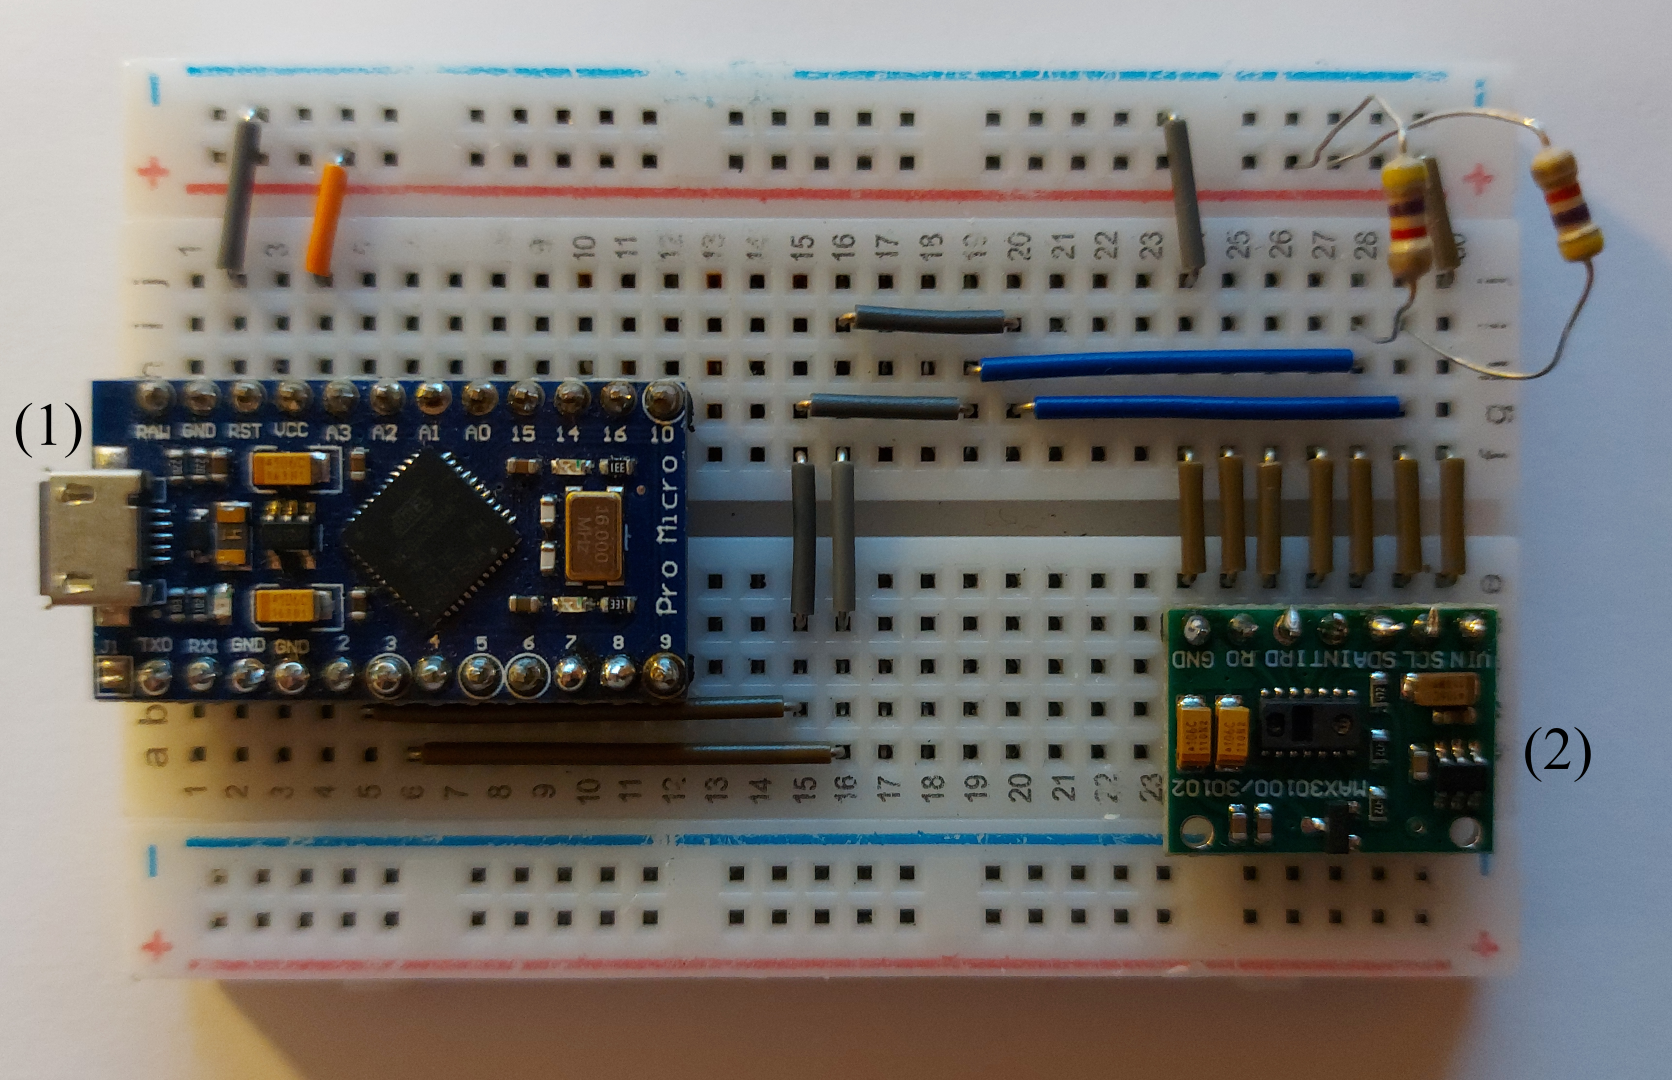
\includegraphics[scale=0.27, center]{Kapitoly/Prakticka/Obrazky/První_prototypy.png}
  \caption [První prototyp]{Takto vypadaly první prototypy. (1) je jednodeskový mikroprocesor a (2) je oxymetr.}
  \label{fig:První_prototyp}
\end{figure}
Nejjednodušší způsob, jak udělat první prototyp, je ke všem součástkám se kterými je v plánu pracovat, připájet piny a začít stavět na nepájivém poli. Naše první prototypy obsahovaly křemíkovou fotodiodu, dvě LED o vlnových délkách 640 a 940 nm a pomocné obvody pro měření s již zmíněnou fotodiodou. Také ještě používaly jednodeskové mikroprocesory stavěné na designech od společnosti Arduino a běžících na 5 V. Pomocí diod jsme se u těchto prototypů snažili naměřit co nejvíc dat. Dařilo se nám měřit pomocí obou zdrojů světla a z naměřených dat byl jednoduše získatelný samotný tep. U dalších prototypů jsme ale již začali experimentovat s oxymetry postavenými na MAX30100, které ještě budou zmíněny. Prototyp s MAX30100 jde vidět na obrázku \ref{fig:První_prototyp}. V dalších verzích tohoto prototypu byl hlavní cíl zjišťovat vhodnost jednotlivých součástek pro naše využití a vyzkoušet, zda fungují.
\paragraph{MAX30100}
Jako samotný oxymetr jsme se rozhodli použít MAX30100, který je jedním z nejčastějších komerčně dostupných oxymetrů na trhu. \citep{max30100}. Plošný spoj, na kterém se MAX30100 nachází, již obsahuje všechny důležité podpůrné komponenty: převodníky napětí na 3,3 V a 1,8 V (obě napěťové hladiny jsou nutností pro operaci MAX30100), kondenzátory a rezistory. Jednou ze zajímavých vlastností designu těchto desek jsou i integrované pullup rezistory. Tyto rezistory jsou na $I^2C$ sběrnici a propojují ji s 1,8 V, což pro naše využití bohužel není užitečná vlastnost. To, že tyto rezistory nejsou pro námi používaná zařízení dostatečné, znamená že si musíme připojit vlastní, které budou sběrnici spojovat s dostatečně vysokým napětím, což jsou v našem případě 3,3 V, na kterých běží i samotný procesor. Zbývá již jen poslední otázka, a to zda tam lze tyto zbytečné rezistory nechat. Odpovědí je, že v našem případě ano, ale je potřeba si dávat pozor, protože i na první pohled zcela nesouvisející změny by mohly odpověď na tuto otázku změnit na ne. Záludnost tohoto problému spočívá v tom, že tyto dva páry pullupových rezistorů tvoří napěťový dělič mezi 1,8 V a naším napájecím napětím (3,3 V), který ústí do naší sběrnice. V našem případě (4,7kΩ pullupové rezistory, Pi Pico a napájecí napětí 3,3 V) tento dělič vytvoří napětí 2,55 V, což je s rezervou více, než 2 V, které Pi Pico bere jako logickou hodnotu 1. To samé platí u samotného oxymetru a displeje, u nichž je naštěstí ještě vyšší rezerva. Problém by ale mohl nastat již při připojení dalšího zařízení na sběrnici, které by tyto podmínky nemuselo zvládat, nebo výměny jednoho ze stávajících zařízení za jiné kompatibilní (třeba jiný mikrokontroler, nebo displej). Proto nemusí být špatný nápad rezistory pro jistotu odstranit, což jsme na našich prototypech také udělali.
\subsubsection {Druhý prototyp}
Účelem druhého prototypu bylo jednak vyřešit problémy které dělalo okolní světlo oxymetru při měření, a také postavit takový prototyp, který by byl více reprezentativním testem pro finální verzi.
\begin{figure}[ht]
  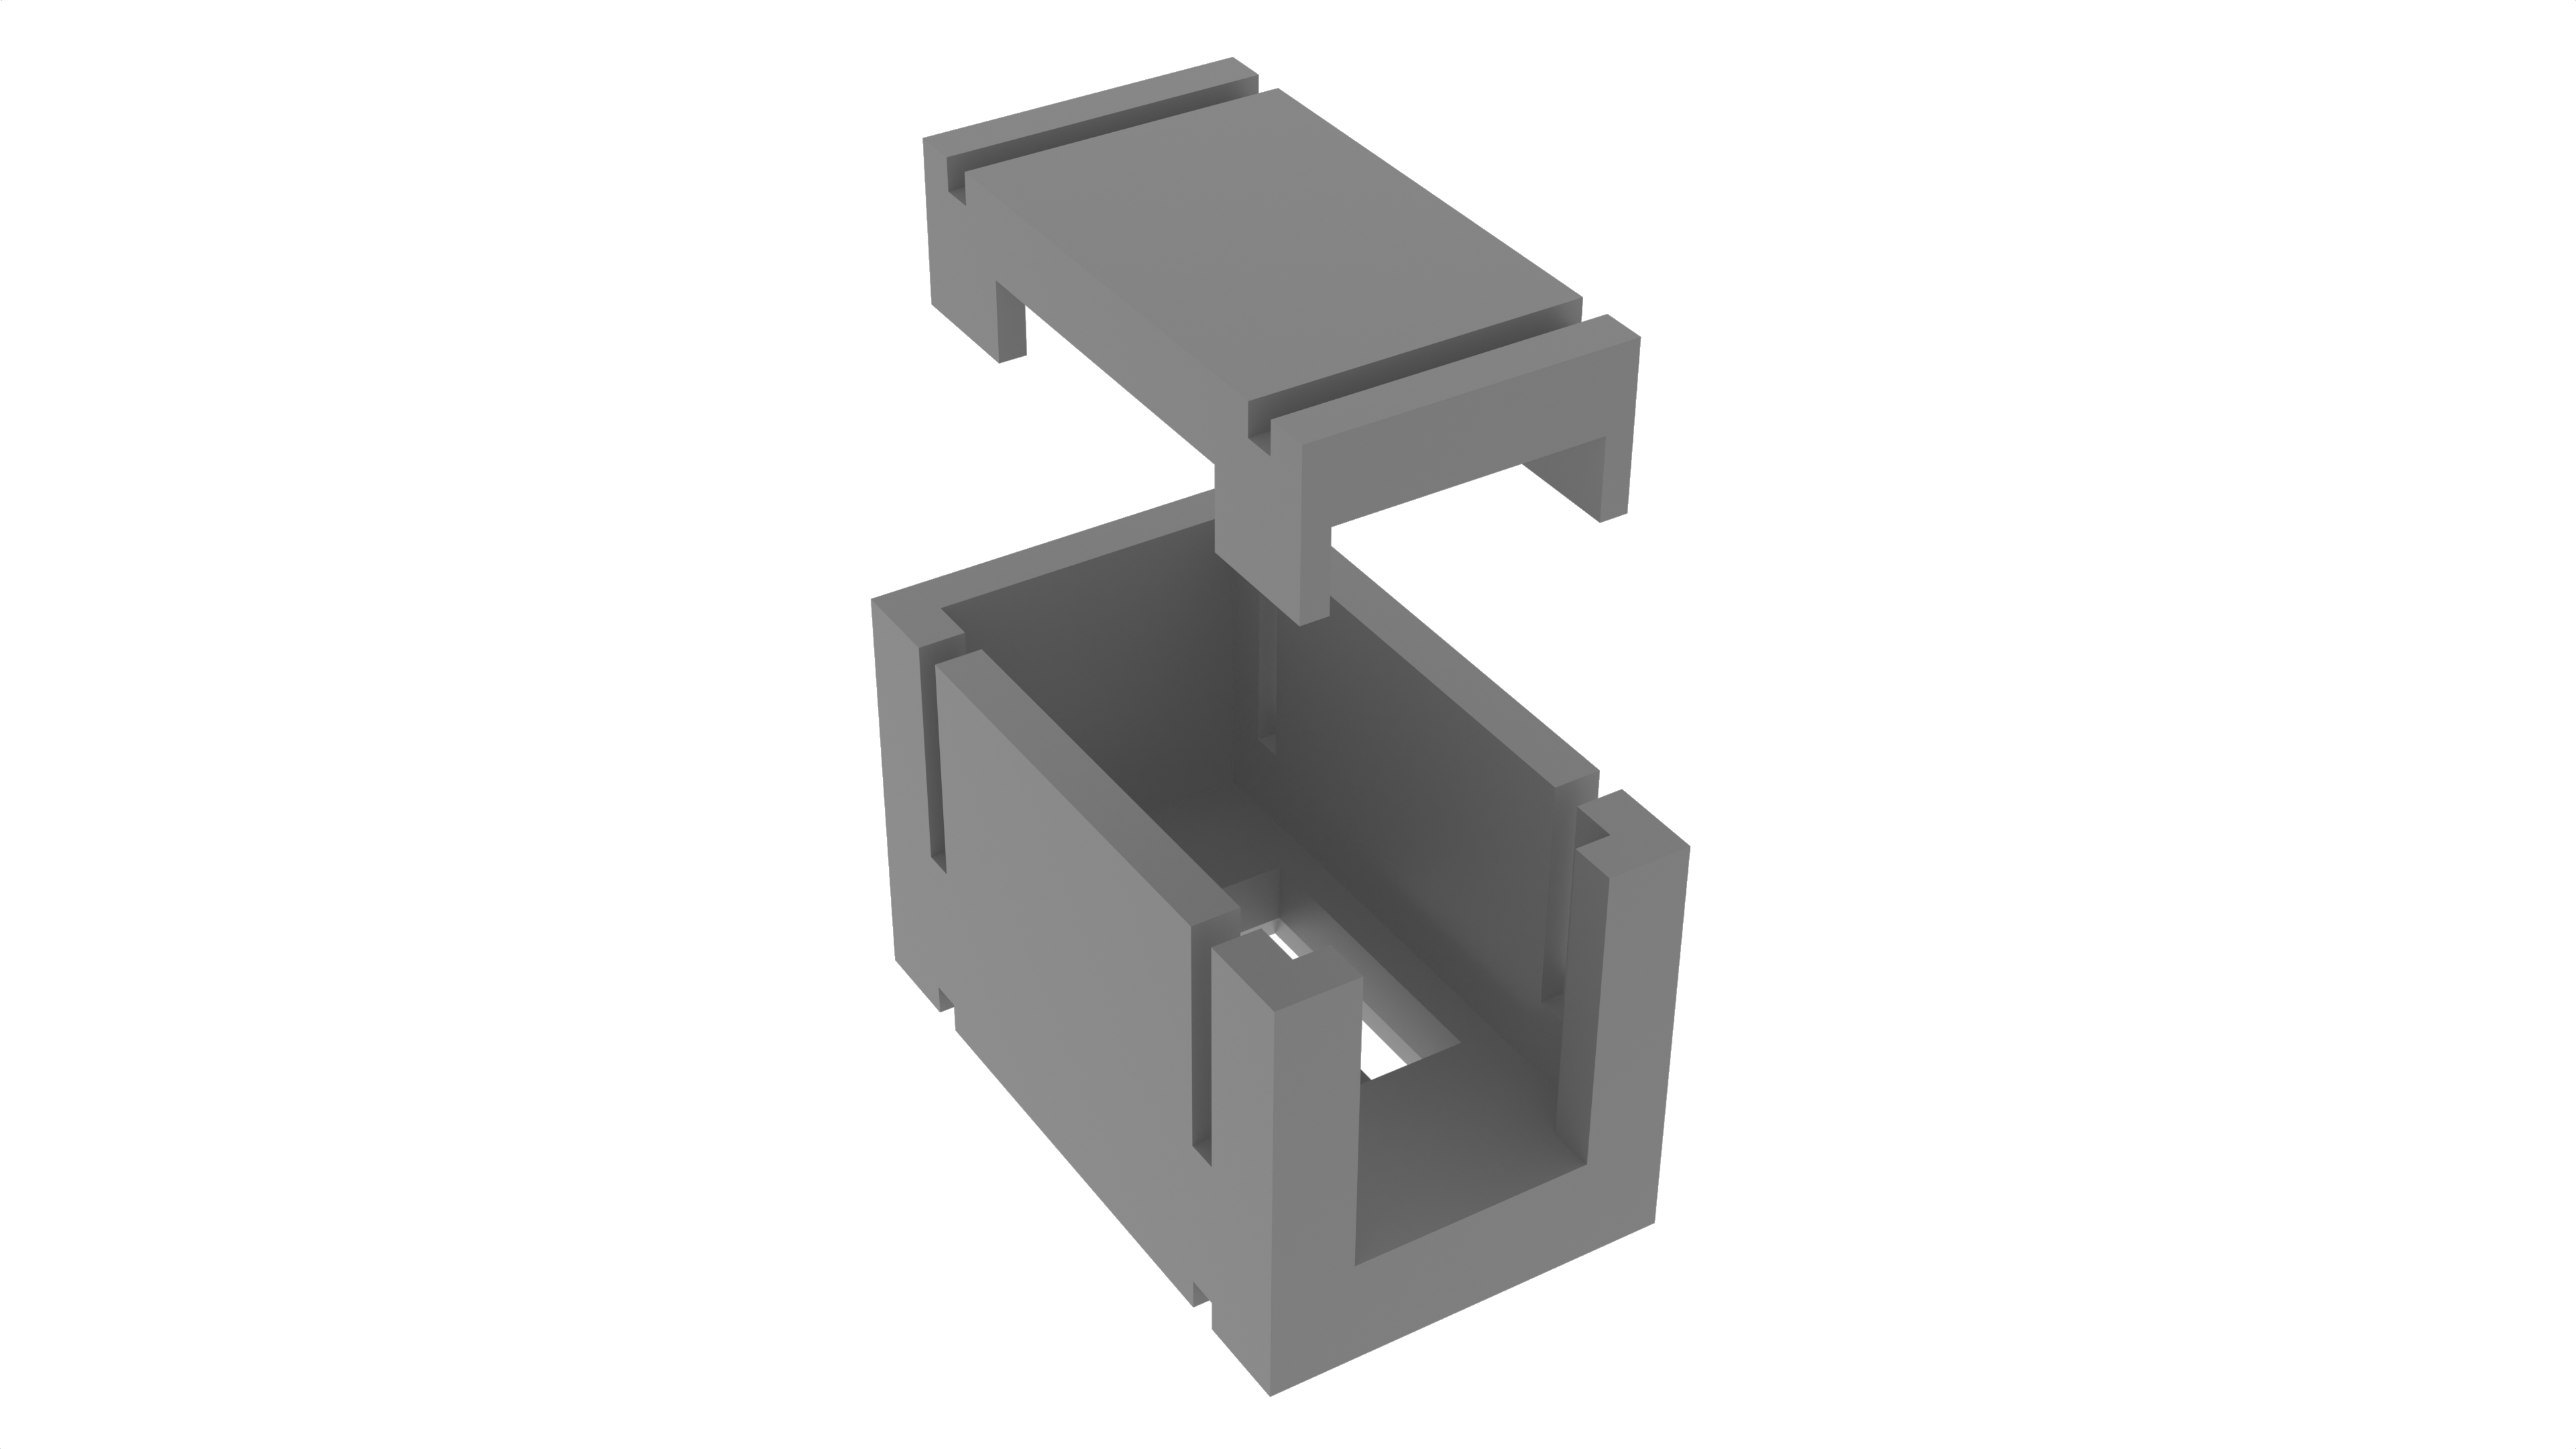
\includegraphics[scale=0.13, center]{Kapitoly/Prakticka/Obrazky/Druhý_prototyp2_w.png}
  \caption [3D model druhého prototypu]{3D tištěná část druhého prototypu. Skládá se jen ze dvou částí – spodní komory pro prst, která obsahuje i místo pro destičku s oxymetrem a horní části která má za úkol pomocí gumičky komoru seshora i s prstem uzavřít.}
  \label{fig:3D_model_druhého_prototypu}
\end{figure}
\paragraph{3D tisk / Modelování}
Tento první model se nakonec skládal jen ze dvou částí: spodní komory pro prst obsahující i místo pro destičku s oxymetrem a horní části, která měla za úkol pomocí gumičky komoru ze shora i s prstem uzavřít. Tento design se ukázal býti efektivním a zajistil spolehlivé měření. Tento design je převážně dílem Benjamina Swarta a pomohl nám při modelování všech ostatních modelů, které jsou naši úpravou tohoto modelu. Všechny ostatní modely jsou upravenou verzí tohoto a všechny úpravy jsou již dělány námi.
\subsubsection {Finální verze}
Informace získané z druhého prototypu jsme zúročili při návrhu finálního výrobku, který již spojuje nejen samotné Pi Pico a destičku oxymetru, ale i akumulátor se všemi svými podpůrnými obvody a ovládacími prvky. Má velkou spodní část, kde se schovají všechny elektronické obvody.
\begin{figure}[ht]
  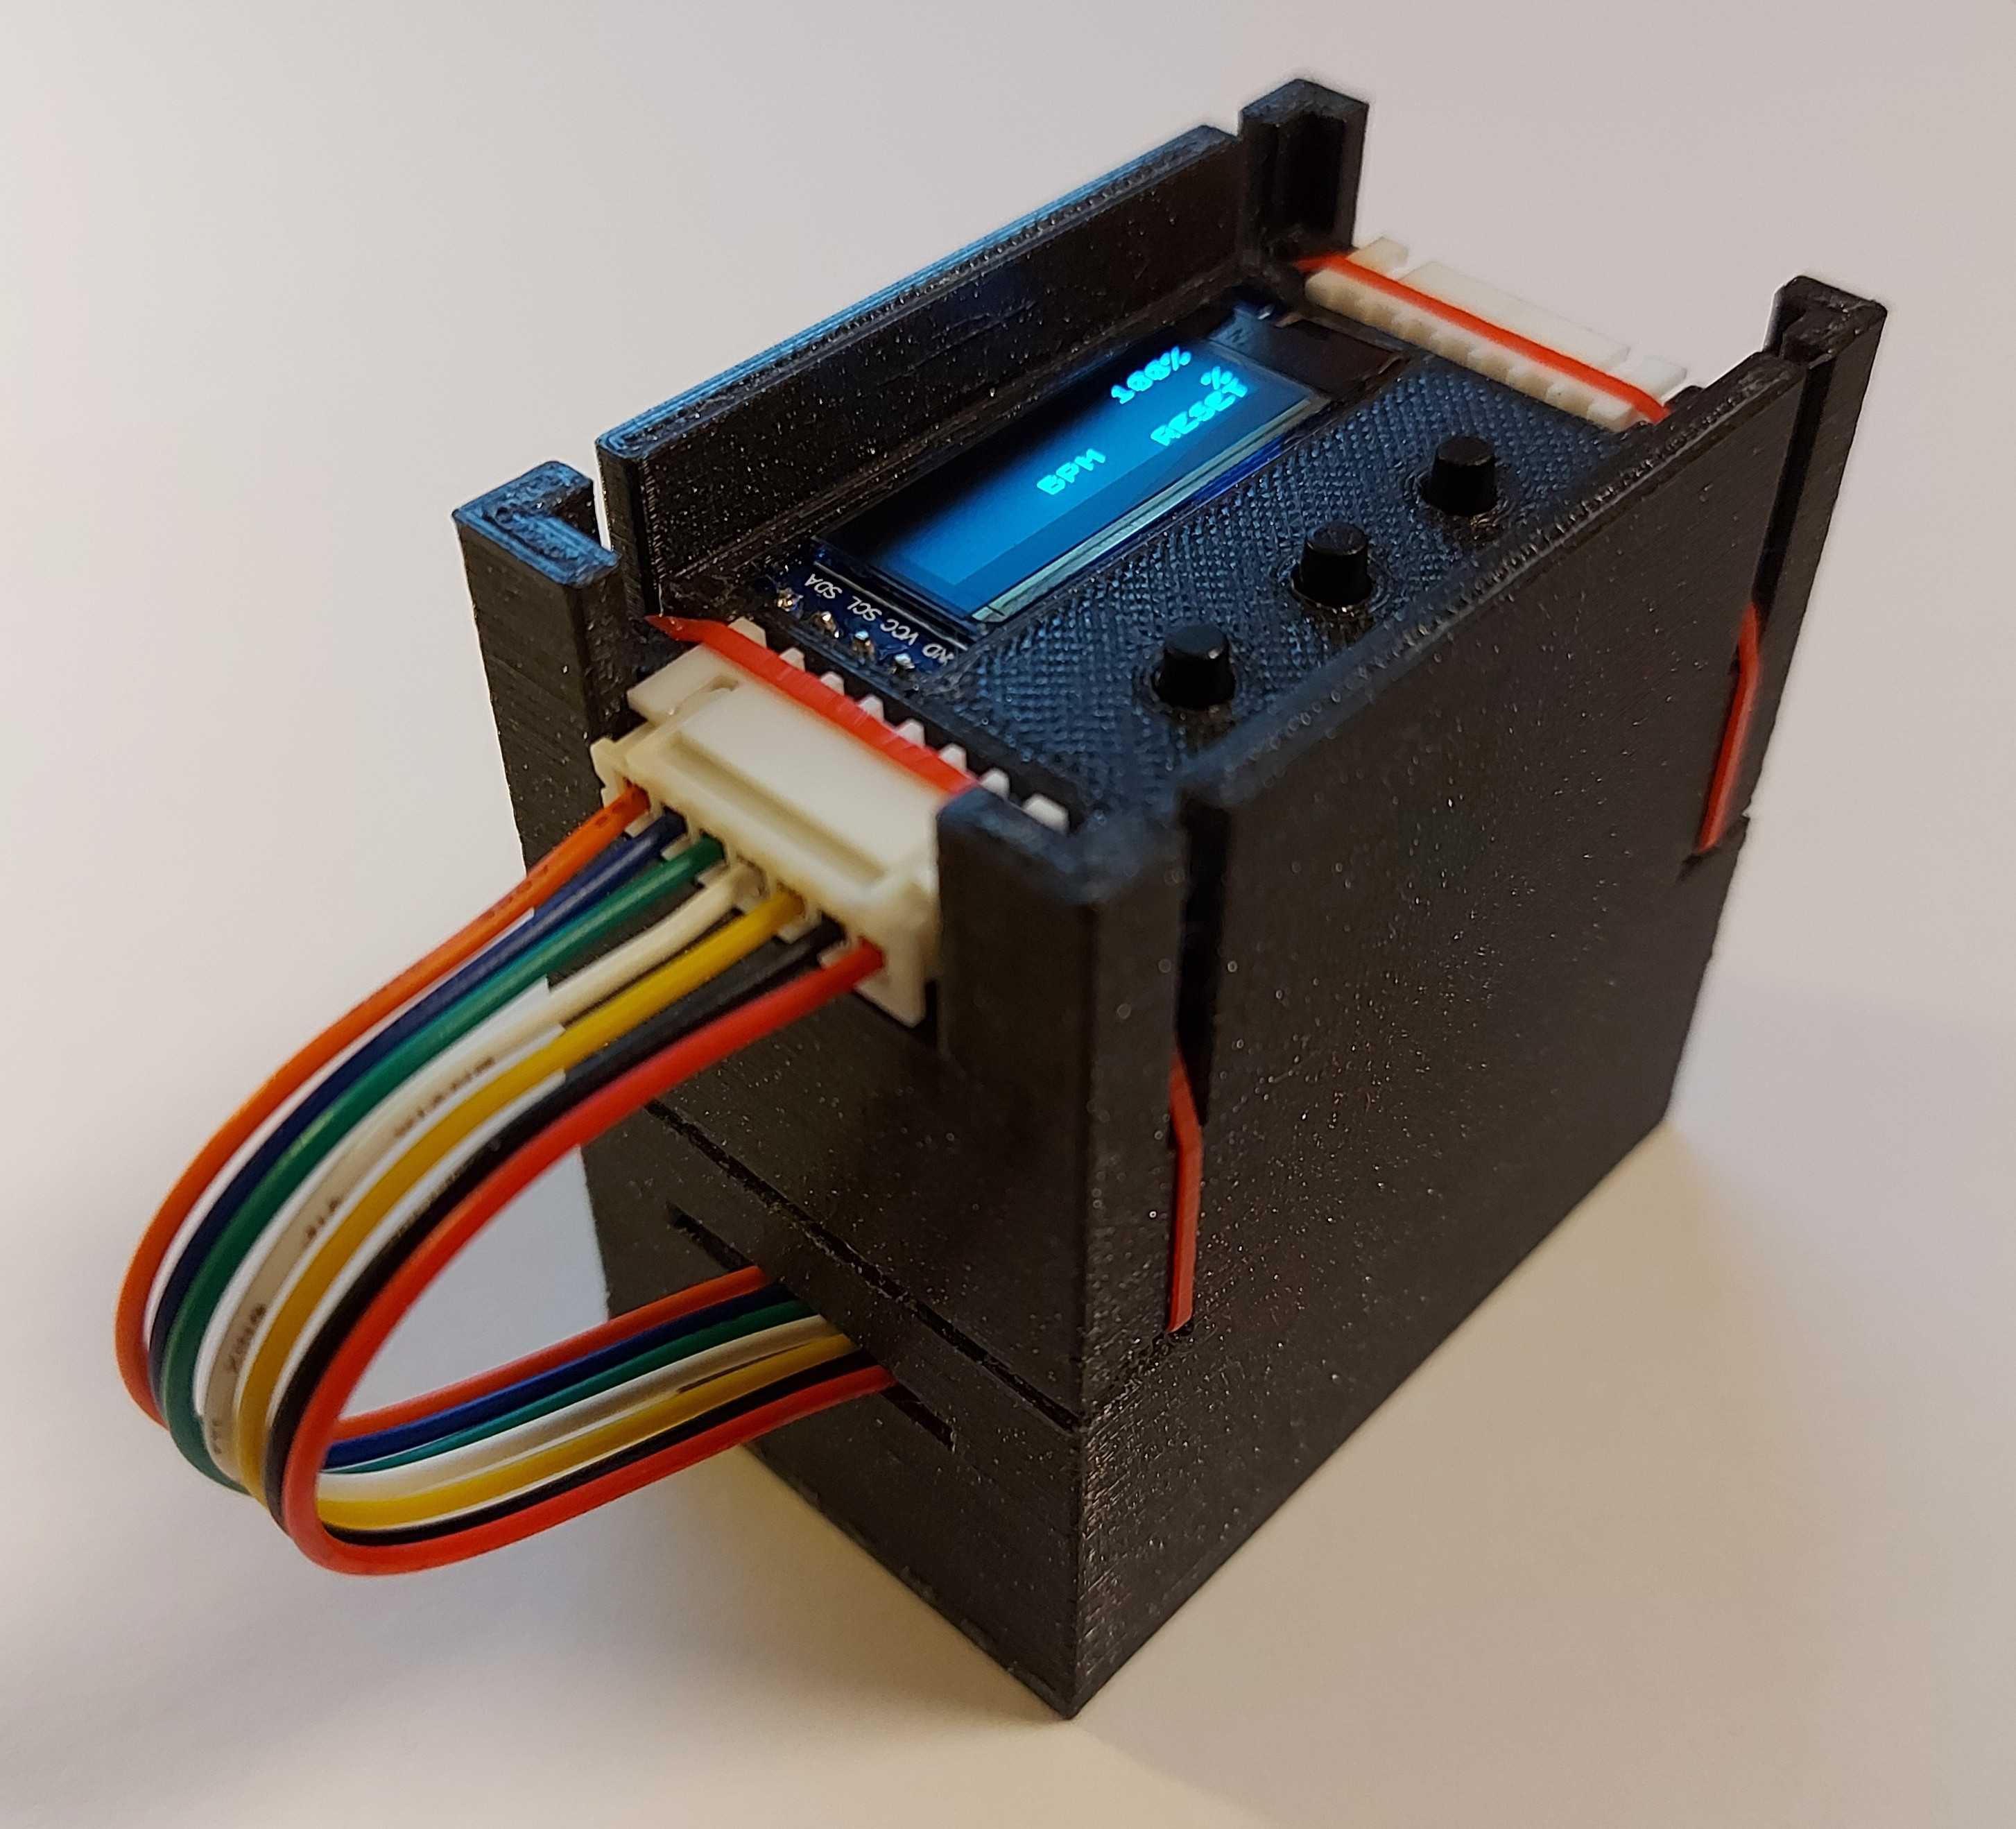
\includegraphics[scale=0.12, center]{Kapitoly/Prakticka/Obrazky/Finální_prototyp.jpg}
  \caption [Finální prototyp]{Hotový pulzní oxymetr v pohledu zprava zezadu.}
  \label{fig:Finální_prototyp}
\end{figure}
\begin{figure}[ht]
  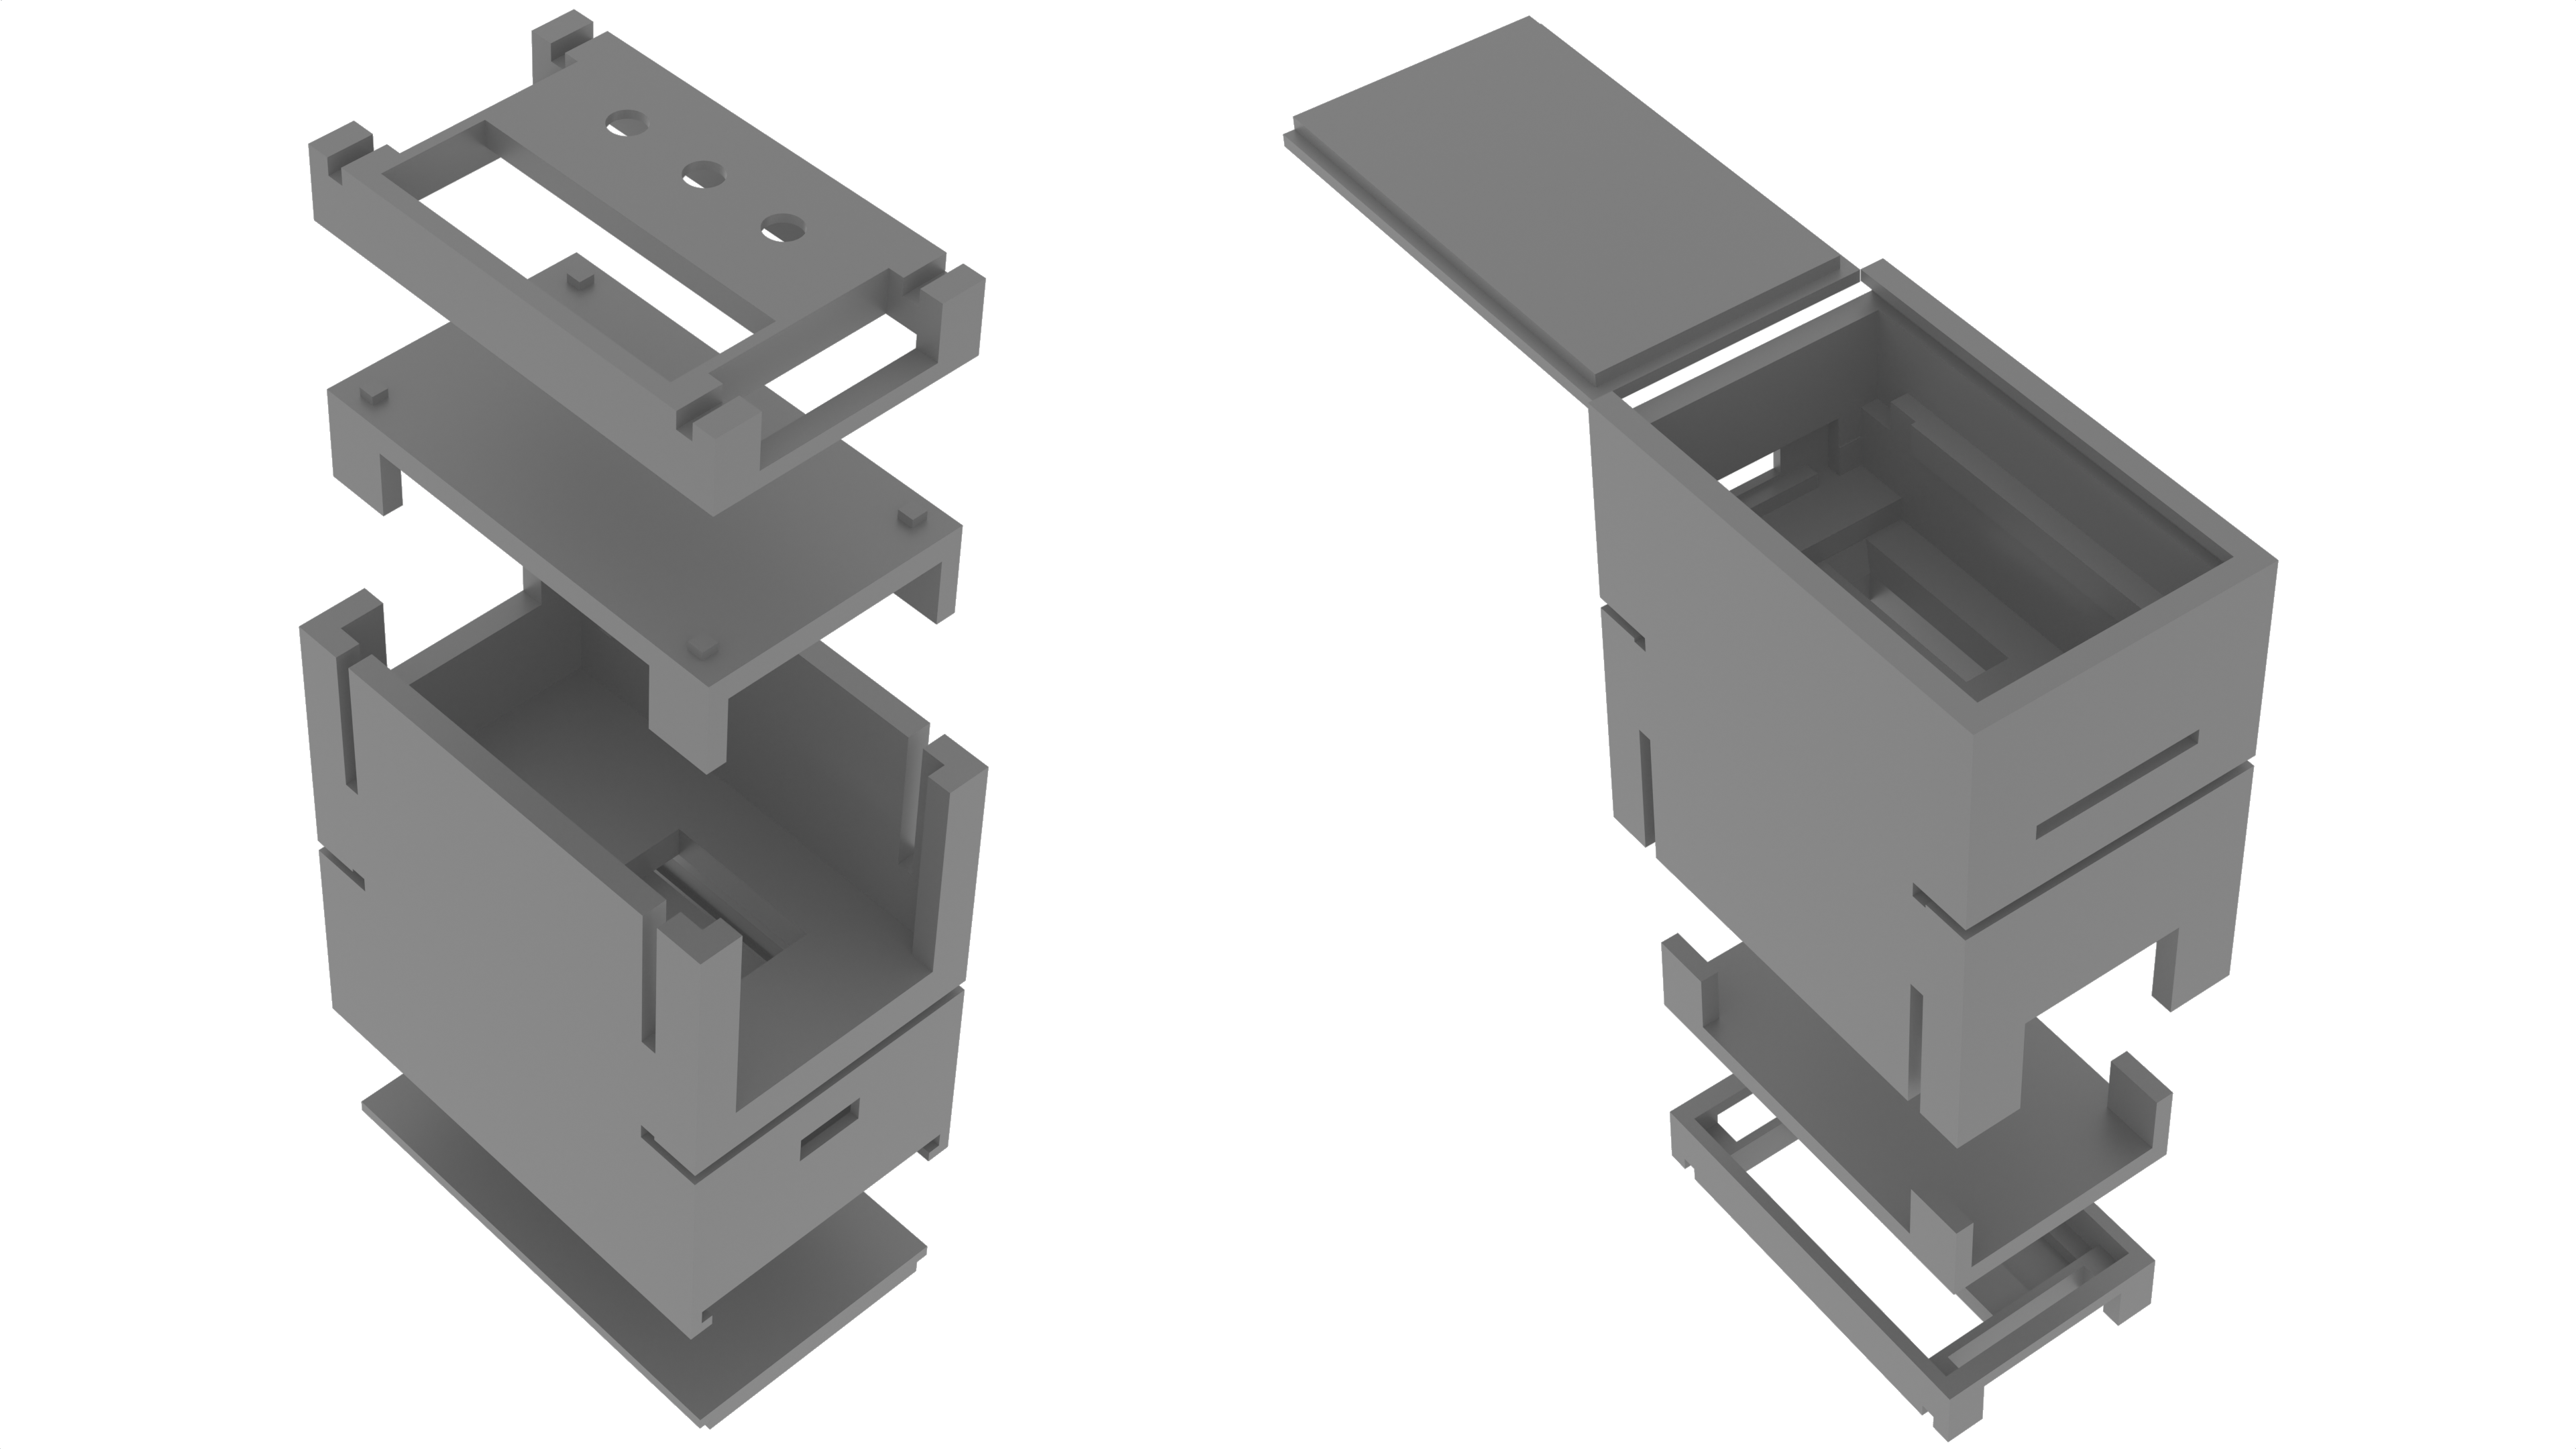
\includegraphics[scale=0.13, center]{Kapitoly/Prakticka/Obrazky/Finální.png}
  \caption [3D model finálního prototypu]{3D model finálního prototypu, který již obsahuje spodní komoru pro prst a destičku s oxymetrem rozšířenou o místo pro ovládací a napájecí elektroniku a místo pro samotný akumulátor, dvířka pro zavření místa pro elektroniku a horní část která se skládá ze dvou kusů, aby se do ní mohl zavřít plošný spoj s displejem a tlačítky.}
  \label{fig:3D_model_finálního_prototypu}
\end{figure}
\paragraph{Nový model}
Design tohoto prototypu začal pečlivým měřením všech součástek a stavěním samotného 3D modelu. Při tomto procesu bylo velmi důležité dát si pozor, aby všude byly dostatečné rezervy.
\paragraph{Displej a tlačítka}
Problémem bylo i umístnění displeje a ovládacích tlačítek. Design oxymetru bohužel neumožňuje jednoduché umístění ovládacích prvků na horní stranu, protože žádná volná horní strana neexistuje. Jedním z jediných jednoduchých řešení je dát displej z boku samotného oxymetru. Toto řešení jsme ale zamítli, a to proto, že by nebylo pohodlné při používání zařízení. Jedním z důvodů tohoto zamítnutí je obecná nešikovnost místa, vzhledem k tomu že na tom místě budou pravděpodobně překážet prsty. Navíc by v tuto chvíli potřebné naklánění oxymetru a tlačení na něj ze strany mohlo ovlivnit měření dat. Druhým z důvodů je to, že pokud je displej na jedné straně oxymetru, je relativně pohodlné ovládání na jedné z rukou, avšak by bylo náročné používat ho na té druhé, a to jednoduše proto, že by displej mířil pryč od samotného uživatele. Řešení, které jsme nakonec použili je displej a tlačítka vestavět do samotné horní posuvné části oxymetru a propojit se zbytkem kabely vedenými zvenku. Tyto kabely mohou být odpojeny a připojeny z druhé strany modulu pro používání na druhé ruce. Toto řešení se ukázalo býti docela elegantním a mělo jedinou malou nevýhodu, a to tu, že to udělalo celý oxymetr větším. To se stalo proto, že kromě samotného displeje, který má nějakou velikost, musí být kolem něj trochu plastu pro udržení struktury, a na obou koncích musí být konektory pro zmíněný propojovací kabel. Tato prostorová limitace ale také znamenala zvětšení prostoru na práci v těle samotného oxymetru. Konkrétně se nám díky tomuto nucenému zvětšení vešel do spodní části větší 900mAh akumulátor.
\begin{figure}[ht]
    \def\svgwidth{\columnwidth}
    \input{Kapitoly/Prakticka/Obrazky/oxymetr.pdf_tex}
    \caption [Schematický diagram obvodu]{Schematický diagram celého obvodu. U1 je samotné Raspberry Pi Pico. Jeho $I^2C$ sběrnice má na sobě 4,7kΩ pullupové rezistory. Tato sběrnice je rovnou připojena k oxymetru (U3), a pomocí sedmipinového konektoru J3 přímo k modulu s displejem. Modul s displejem obsahuje 3 talčítka, z nichž 2 již mají připojeny 10kΩ pulldownové rezistory. Na straně Pica jsou tato tlačítka propojena s GPIO10 a GPIO11 a tlačítko bez rezistoru je připojeno k pinu RUN. K Picu je připojen akumulátor, a to skrz jeho nabíjecí a ochraný modul a Schottkyho diodu.}
    \label{fig:Diagram}
\end{figure}
\subsection {Software}
Nedílnou součástí našeho oxymetru je i jeho software. Hlavní dvě věci, které musí software dělat je komunikovat s našimi dvěma $I^2C$ zařízeními. Toto se děje po jedné $I^2C$ sběrnici a je převážně zařizováno knihovnami určenými pro daná zařízení. Pro oxymetr jsme použili knihovnu MAX30100lib, která nejen zařizuje komunikaci, ale také přímo počítá tep a $SpO_2$. Druhým takto připojeným zařízením je displej. Pro komunikaci s ním jsme využili knihovny U8g2. Ta nám dovolila jednoduše zobrazit potřebný text na jakoukoli část displeje. Poslední z komponent určených pro uživatele jsou tlačítka. Jedno z nich je ovládáno na úrovni hardwaru, tím že je připojeno mezi pinem RUN a GND.  Jeho stisknutí způsobí restart. Zbylá dvě tlačítka jsou připojena k pinům GPIO10 a GPIO11 s 10kΩ pullup rezistory a vyžadují softwarové ovládání. Další důležitou funkcí je část kódu, která pomocí měření vstupního napětí z akumulátoru odhaduje kolik v něm ještě zbývá energie, nebo, v případě že je Pi Pico zrovna připojené k externímu zdroji, o tom podává informaci. Poslední skrytou funkcí je možnost zaznamenávat (a následně z počítače stáhnout) naměřená data. Data se zaznamenávají automaticky od zapnutí do velkého seznamu. Po připojení k počítači je poté možné sériovou linkou poslat příkaz „D“, který když Pi Pico dostane, vypíše všechna data která zatím naměřilo. Tohoto lze dosáhnout automaticky pomocí programu v Pythonu, který z takto získaných dat automaticky vytvoří CSV soubor.